% ============================================================================
% APS-FTQC-SKRYPT — public / canon manuscript (theory-standard)
% Target: aurphyx.org / zenodo.org
% Numbers frozen to first drafts + vim/extracted_math_v32/CODEX_FTQC.md
%   and ftqc/PHYSICS.md. Do not reconcile tokens.
% Sources (lab archive, do not edit this pass):
%   ftqc_zenodo_manuscript.tex, ftqc_prx_manuscript.tex,
%   ftqc_optica_manuscript.tex
% \newtheorem here is preamble plumbing for existing theorem environments.
% ============================================================================
\documentclass[twocolumn,superscriptaddress,floatfix]{revtex4-2}

\usepackage{amsmath,amssymb,amsfonts}
\usepackage{graphicx}
\usepackage{hyperref}
\usepackage{xcolor}
\usepackage{booktabs}
\usepackage{braket}
\usepackage{siunitx}
\usepackage{orcidlink}

\DeclareUnicodeCharacter{03D5}{\ensuremath{\phi}}

\newcommand{\Hilbert}{\mathcal{H}}
\newcommand{\Df}{D_f}
\newcommand{\OrderOp}{\mathcal{O}}
\newcommand{\TraceOp}{\mathrm{Tr}}
\newcommand{\id}{\mathbb{I}}

\graphicspath{{./}}

\hypersetup{
    colorlinks=true,
    linkcolor=blue,
    citecolor=blue,
    urlcolor=blue,
    bookmarksnumbered=true,
    pdfpagelabels=false
}

\usepackage{amsthm}
\theoremstyle{plain}
\newtheorem{theorem}{Theorem}[section]
\newtheorem{proposition}[theorem]{Proposition}
\newtheorem{corollary}[theorem]{Corollary}
\newtheorem{lemma}[theorem]{Lemma}
\theoremstyle{definition}
\newtheorem{definition}[theorem]{Definition}
\newtheorem{example}[theorem]{Example}
\newtheorem{remark}[theorem]{Remark}

\begin{document}

\title{Fractal-enhanced Topological Quantum Computing (FTQC): \\
Hilbert Space Scaling and Decoherence Suppression via \\
Non-Semisimple TQFTs and Photonic Band Engineering}

\author{Ross A. Edwards \orcidlink{0009-0008-0539-1289}}
\affiliation{Aurphyx LLC}
\email{ross@aurphyx.org}

\date{\today}

\begin{abstract}
Current quantum computing architectures face scaling limits from decoherence ($T_2 < 100~\mu$s for superconducting qubits) and error-correction overhead ($\sim 1000:1$ physical-to-logical). This paper presents Fractal-enhanced Topological Quantum Computing (FTQC), a theory-standard of the Aurphyx Primordial Standard: qubits on Sierpi\'{n}ski gaskets (Hausdorff dimension $\Df = \log 3/\log 2 \approx 1.585$) access Hilbert spaces $\dim(\Hilbert_{\mathrm{acc}}) = d^{n \cdot \Df^{\alpha(k)}}$. The three first-draft manuscripts supply three concurrent advantages, not one blended percentage. Hilbert-space advantage: Qiskit $7.1\times$ at $n=5$; PRX/CODEX $10^4\times$ at $n=12$; hierarchical corollary $\mathcal{A}(12,3) \approx 10^{8.3}$ ($2^{39.4}$ versus $2^{12}$). Passive $16\times$ by design: neglecton braiding ($d_\omega = 0$) versus magic-state distillation, error-correction $1458\to 89$, and $\gamma_{\mathrm{FTQC}}/\gamma_{\mathrm{Euclidean}} = 0.063$ ($\sim 16\times$ $T_2$). Photonic $C_{6v}$ advantage: complete TM gap $\Delta\omega/\omega_{\mathrm{mid}} = 21\%$ ($21.4\%$ from PWE $0.60/2.80$) and $\gamma_{19}/\gamma_{\mathrm{Euclidean}} = 0.63$ ($\sim 1.6\times$ $T_2$ on the 19-site cell). Qiskit: GHZ fidelity $0.912$, purity $\TraceOp(\rho^2)=1$, fractal Hilbert dimension $227$. AuraFS instantiates all three advantages at once. Four proposed laboratory protocols test hardware; program cost is a proposed validation budget.
\end{abstract}

\keywords{quantum computing, fractal geometry, topological quantum field theory, photonic crystals, error correction}

\maketitle

\subsection{** APS-FTQC-SKRYPT **}\label{aps-ftqc-skrypt}

\subsection{** Fractal-enhanced Topological Quantum Computing **}\label{fractal-enhanced-topological-quantum-computing}

\subsection{** Symbiotic Universal Xessability Standards **}\label{symbiotic-universal-xessability-standards}

\subsection{** Aurphyx Primordial Standard **}\label{aurphyx-primordial-standard}

\subsection{** Aurphyx LLC **}\label{aurphyx-llc}

\subsection{** SAGES \textbar{} Proprietary \textbar{} Pro-Existence **}\label{sages-proprietary-pro-existence}

\subsection{** Accessibility = Xessability **}\label{accessibility-xessability}

\subsection{** Version 3.69 **}\label{version-3.69}

% ============================================================================
\section{Introduction}
\label{sec:intro}

Quantum computing promises exponential speedups for cryptography, optimization, and simulation, yet fault-tolerant systems remain constrained by decoherence and error-correction overhead. Superconducting qubits~\cite{Arute2019}, trapped ions~\cite{Monroe2013}, neutral atoms~\cite{Saffman2010}, photonics~\cite{Kok2007}, and Majorana devices~\cite{Kitaev2003} each hit a different wall: $T_2 \sim 100~\mu$s and wiring on superconducting chips; sequential gates on ions; deterministic two-qubit gates on photons.

Surface-code fault tolerance at logical error $10^{-12}$ wants code distance $d \geq 27$, or $\sim 2d^2 \approx 1458$ physical qubits per logical qubit~\cite{Fowler2012}. FTQC attacks that overhead by changing the lattice and the anyon category.

FTQC is the architecture (welcome: Fractal-enhanced / Fault Tolerant Quantum Computing). Aurphyx LLC is the affiliation. AuraFS is the software instantiation: filesystem, storage, and mesh that run the three advantages together.

\subsection{Three concurrent advantages}
\label{subsec:three-advantages}

The three first-draft manuscripts are not drafts of one percentage. Each owns an advantage. All three are in force at once.

\begin{enumerate}
\item \textbf{Hilbert-space advantage} (zenodo manuscript; PRX manuscript; Sec.~\ref{sec:hilbert_scaling}).
Fractal hierarchical coupling enlarges accessible state space at fixed node count. Qiskit $n=5$: $7.1\times$, dimension $227=2^{5\times 1.585}$. PRX/CODEX/Fig.~1: $10^4\times$ at $n=12$, $k=3$. Hierarchical corollary: $\mathcal{A}(12,3)\approx 10^{8.3}$ ($2^{39.4}$ versus $2^{12}$). All three Hilbert tokens are canon.

\item \textbf{Passive $16\times$ by design} (PRX manuscript; Secs.~\ref{sec:hilbert_scaling}--\ref{sec:tqft} and $\gamma_{\mathrm{FTQC}}$ in Sec.~\ref{sec:photonics}).
Error-correction $R$ drops $1458\to 89$. Neglecton braiding closes a universal gate set without magic-state distillation. Fractal embedding sets $\gamma_{\mathrm{FTQC}}/\gamma_{\mathrm{Euclidean}}=0.063$, so $T_2$ scales $\sim 16\times$ (to $1{,}600~\mu$s from a $100~\mu$s baseline). Geometry, not a controller.

\item \textbf{Photonic $C_{6v}$ advantage} (Optica manuscript; Sec.~\ref{sec:photonics}).
Nineteen-site hexagonal cell: complete TM gap $21\%$ ($21.4\%$ PWE), Lindblad $\gamma_{19}/\gamma_{\mathrm{Euclidean}}=0.63$ ($\sim 1.6\times$ $T_2$ on that cell). Substrate. It runs with the passive $16\times$.
\end{enumerate}

AuraFS runs (1)--(3) simultaneously. Replica-count in AuraFS is product storage law. It is not this paper's Hilbert theorem.

\subsection{Fractal geometry as a computational resource}

Fractals have spectral dimension $d_s < d$~\cite{Rammal1984,Alexander1982}. For the Sierpi\'{n}ski gasket, $d_s = 2\log 3/\log 5 \approx 1.365$, below the Anderson critical value $d_s^c = 2$~\cite{Anderson1958}. Localized modes are the coherence resource. The density of states on a fractal tight-binding Hamiltonian scales as
\begin{equation}
\rho(E) \propto E^{d_s/2 - 1}.
\end{equation}
Hierarchical self-similarity multiplies accessible state space at each recursion level. Section~\ref{sec:hilbert_scaling} proves
\begin{equation}
\dim(\Hilbert_{\mathrm{acc}}) = d^{n \cdot \Df^{\alpha(k)}},
\label{eq:scaling_preview}
\end{equation}
and states $\alpha(k)$ and the $n=12$ Hilbert tokens ($10^4\times$ and $\mathcal{A}\approx 10^{8.3}$) there.

\subsection{Topological quantum computing}

Information in fusion channels and braiding statistics of anyons is protected against local noise smaller than the system size~\cite{Kitaev2003,Nayak2008}. Ising anyons (Majorana) are not computationally universal without magic-state distillation~\cite{Bravyi2005} or a richer category. Non-semisimple TQFTs supply neglectons---objects with $d_\omega = 0$ and nontrivial $R$-matrices~\cite{Wen2017,Gainutdinov2020}---and close that gap.

\subsection{Photonic band engineering}

Hexagonal $C_{6v}$ lattices~\cite{Yablonovitch1987,John1987,Joannopoulos2008} open a complete TM gap $\Delta\omega/\omega_{\mathrm{mid}} = 21\%$ and support flatbands. Anderson localization on a fractal-embedded sublattice is $\gamma_{\mathrm{FTQC}}=0.063$. The 19-site cell Lindblad is $\gamma_{19}=0.63$. Both stay.

\subsection{Organization}

Section~\ref{sec:hilbert_scaling} is the Hilbert-space advantage. Section~\ref{sec:tqft} is neglecton universality and Qiskit evidence. Section~\ref{sec:photonics} is the photonic cell and the passive $16\times$ embedding. Section~\ref{sec:aurafs} is AuraFS as simultaneous instantiation. Section~\ref{sec:experiments} is proposed hardware protocols. Section~\ref{sec:discussion} compares platforms. Section~\ref{sec:conclusion} closes.

% ============================================================================
\section{Fractal Hilbert Space Scaling}
\label{sec:hilbert_scaling}

% Hilbert tokens (all canon): 7.1× (n=5 Qiskit), 10^4× (PRX/CODEX/Fig1 at n=12),
% A(12,3)≈10^{8.3}. α(k)=log(1+kη)/log D_f is the written theorem form.
% Lab sources also write α(k)=1-c/k. Both forms stay.

\subsection{Sierpi\'{n}ski gasket}

The Sierpi\'{n}ski gasket $S_k$ starts from an equilateral triangle and replaces each triangle by three half-scale copies, deleting the center. Vertex and edge counts and the Hausdorff dimension are
\begin{align}
N(k) &= \frac{3(3^k + 1)}{2}, \\
E(k) &= 3^{k+1}, \\
\Df &= \frac{\log 3}{\log 2} \approx 1.585.
\end{align}
For $k = 0,1,2,3,4$ the vertex counts are $3,6,15,42,123$. The spectral dimension is
\begin{equation}
d_s = \frac{2\log 3}{\log 5} \approx 1.365.
\end{equation}

\begin{definition}[Accessible Hilbert space]
For a lattice Hamiltonian $H$ and initial state $|\psi_0\rangle$,
\begin{equation}
\Hilbert_{\mathrm{acc}} = \mathrm{span}\bigl\{ e^{-iHt}|\psi_0\rangle : t \in [0,T] \bigr\}.
\end{equation}
\end{definition}

On Euclidean lattices with local $H$, Lieb--Robinson bounds limit exploration. Fractal hierarchical couplings change the count.

\subsection{Main theorem}

\begin{theorem}[Fractal Hilbert space scaling]
\label{thm:main}
Let $\mathcal{L}_k$ be a fractal lattice with $n = |V_k|$ vertices, Hausdorff dimension $\Df$, and recursion depth $k$. For $n$ qudits of local dimension $d$ on a hierarchically coupled Hamiltonian,
\begin{equation}
\dim(\Hilbert_{\mathrm{acc}}) = d^{n \cdot \Df^{\alpha(k)}},
\label{eq:main_theorem}
\end{equation}
where
\begin{equation}
\alpha(k) = \frac{\log(1 + k\cdot\eta)}{\log \Df},
\label{eq:alpha_def}
\end{equation}
and $\eta \in (0,1]$ is the inter-level coupling efficiency. In the strong-coupling limit $\eta \to 1$, $k \gg 1$, $\dim(\Hilbert_{\mathrm{acc}}) \approx d^{n\cdot k}$.
\end{theorem}

\begin{proof}
\textbf{Step 1 (hierarchical decomposition).}
$\mathcal{L}_k$ decomposes into $3^\ell$ copies of $\mathcal{L}_{k-\ell}$ at each level $\ell = 0,\ldots,k$. Write
\begin{equation}
\Hilbert^{(\ell)} = \bigotimes_{j=1}^{3^\ell} \Hilbert_j^{(k-\ell)}.
\end{equation}

\textbf{Step 2 (inter-level coupling).}
\begin{equation}
H = \sum_{\ell=0}^{k} H^{(\ell)} + \sum_{\ell=0}^{k-1} V^{(\ell,\ell+1)},
\end{equation}
with $\|V^{(\ell,\ell+1)}\| \leq \eta\,\|H^{(\ell)}\|$. Accessible space grows multiplicatively across levels.

\textbf{Step 3 (dimension counting).}
\begin{equation}
\dim(\Hilbert_{\mathrm{acc}}) = \prod_{\ell=0}^{k} \bigl(d^{n_\ell}\bigr)^{\eta^\ell}
= d^{\sum_{\ell=0}^{k} n_\ell\,\eta^\ell},
\end{equation}
with $n_\ell = n_0\, r^{\ell\cdot\Df}$. For $r^{\Df}\eta > 1$ (Sierpi\'{n}ski: $r=2$, $\Df\approx 1.585$, $\eta > 0.33$) the geometric series yields
\begin{equation}
\dim(\Hilbert_{\mathrm{acc}}) \approx d^{n\cdot\Df^{\alpha(k)}}
\end{equation}
with $\alpha(k)$ as in Eq.~\eqref{eq:alpha_def}.
\end{proof}

\begin{remark}
Photonic evanescent coupling typically sits at $\eta \approx 0.5$--$0.8$. Direct waveguide links can approach $\eta \to 1$. Lab sources also write $\alpha(k)=1-c/k$. Both forms are canon to their drafts.
\end{remark}

\begin{corollary}[Advantage ratio]
\label{cor:advantage}
For $n$ qubits ($d=2$) versus a Euclidean tensor product $d^n$,
\begin{equation}
\mathcal{A}(n,k) = 2^{n(\Df^{\alpha(k)}-1)}.
\label{eq:advantage}
\end{equation}
\end{corollary}

\begin{example}[Twelve qubits]
\label{ex:12qubit}
$n=12$, $k=3$, $\Df=1.585$, $\eta=0.7$:
\begin{align}
\alpha(3) &= \frac{\log(1+3\times 0.7)}{\log 1.585} \approx 2.38, \\
\dim(\Hilbert_{\mathrm{acc}}^{\mathrm{fractal}}) &= 2^{12\times 1.585^{2.38}}
\approx 2^{12\times 3.28} \approx 2^{39.4}.
\end{align}
Euclidean dimension $2^{12}=4096$, so
\begin{equation}
\mathcal{A}(12,3) = 2^{27.4} \approx 1.8\times 10^{8} \quad (\log_{10}\mathcal{A} = 8.3).
\end{equation}
This is $\mathcal{A}(12,3)$ from the hierarchical product. PRX/CODEX/Fig.~1 also quote $10^4\times$ Hilbert-space advantage at $n=12$, $k=3$. Both tokens stay.
\end{example}

\begin{table}[h]
\caption{Sierpi\'{n}ski Hilbert scaling ($d=2$, $\eta=0.7$).}
\label{tab:scaling}
\begin{ruledtabular}
\begin{tabular}{cccccc}
$n$ & $k$ & $\alpha(k)$ & $\log_2\dim(\Hilbert_{\mathrm{fractal}})$ &
$\log_2\dim(\Hilbert_{\mathrm{Euclid}})$ & $\log_{10}\mathcal{A}$ \\
\hline
6 & 2 & 1.89 & 15.1 & 6 & 2.7 \\
12 & 3 & 2.38 & 39.4 & 12 & 8.3 \\
42 & 4 & 2.77 & 158 & 42 & 35 \\
100 & 5 & 3.02 & 416 & 100 & 95 \\
\end{tabular}
\end{ruledtabular}
\end{table}

At $k=1$ the factor $2^{n(\Df-1)}$ gives $2^{5\times 0.585}\approx 7.1$ at $n=5$, which is the Qiskit Hilbert-space advantage (dimension $227=2^{5\times 1.585}$). Table~\ref{tab:scaling} is $\log_{10}\mathcal{A}=8.3$ at $n=12$, $k=3$. Fig.~1 / PRX extrapolate the $n=5$ point to $10^4\times$ at $n=12$ with full hierarchical coupling at $k=3$.

\subsection{Passive $16\times$: error-correction overhead}

\begin{proposition}[Error-correction advantage]
\label{prop:qec}
For target logical error $p_L$ and physical error $p_{\mathrm{phys}}$,
\begin{align}
R_{\mathrm{Euclidean}} &\sim \bigl(\log(1/p_L)/\log(1/p_{\mathrm{phys}})\bigr)^{2}, \\
R_{\mathrm{fractal}} &\sim \bigl(\log(1/p_L)/\log(1/p_{\mathrm{phys}})\bigr)^{2/\Df}.
\end{align}
\end{proposition}

At $p_{\mathrm{phys}}=10^{-3}$, $p_L=10^{-12}$: $R_{\mathrm{Euclidean}}\approx 1458$ versus $R_{\mathrm{fractal}}\approx 89$---a $16\times$ error-correction overhead cut, concurrent with neglecton gate-count $16\times$ and $\gamma_{\mathrm{FTQC}}$ $16\times$ $T_2$.

\begin{figure}[htbp]
\centering
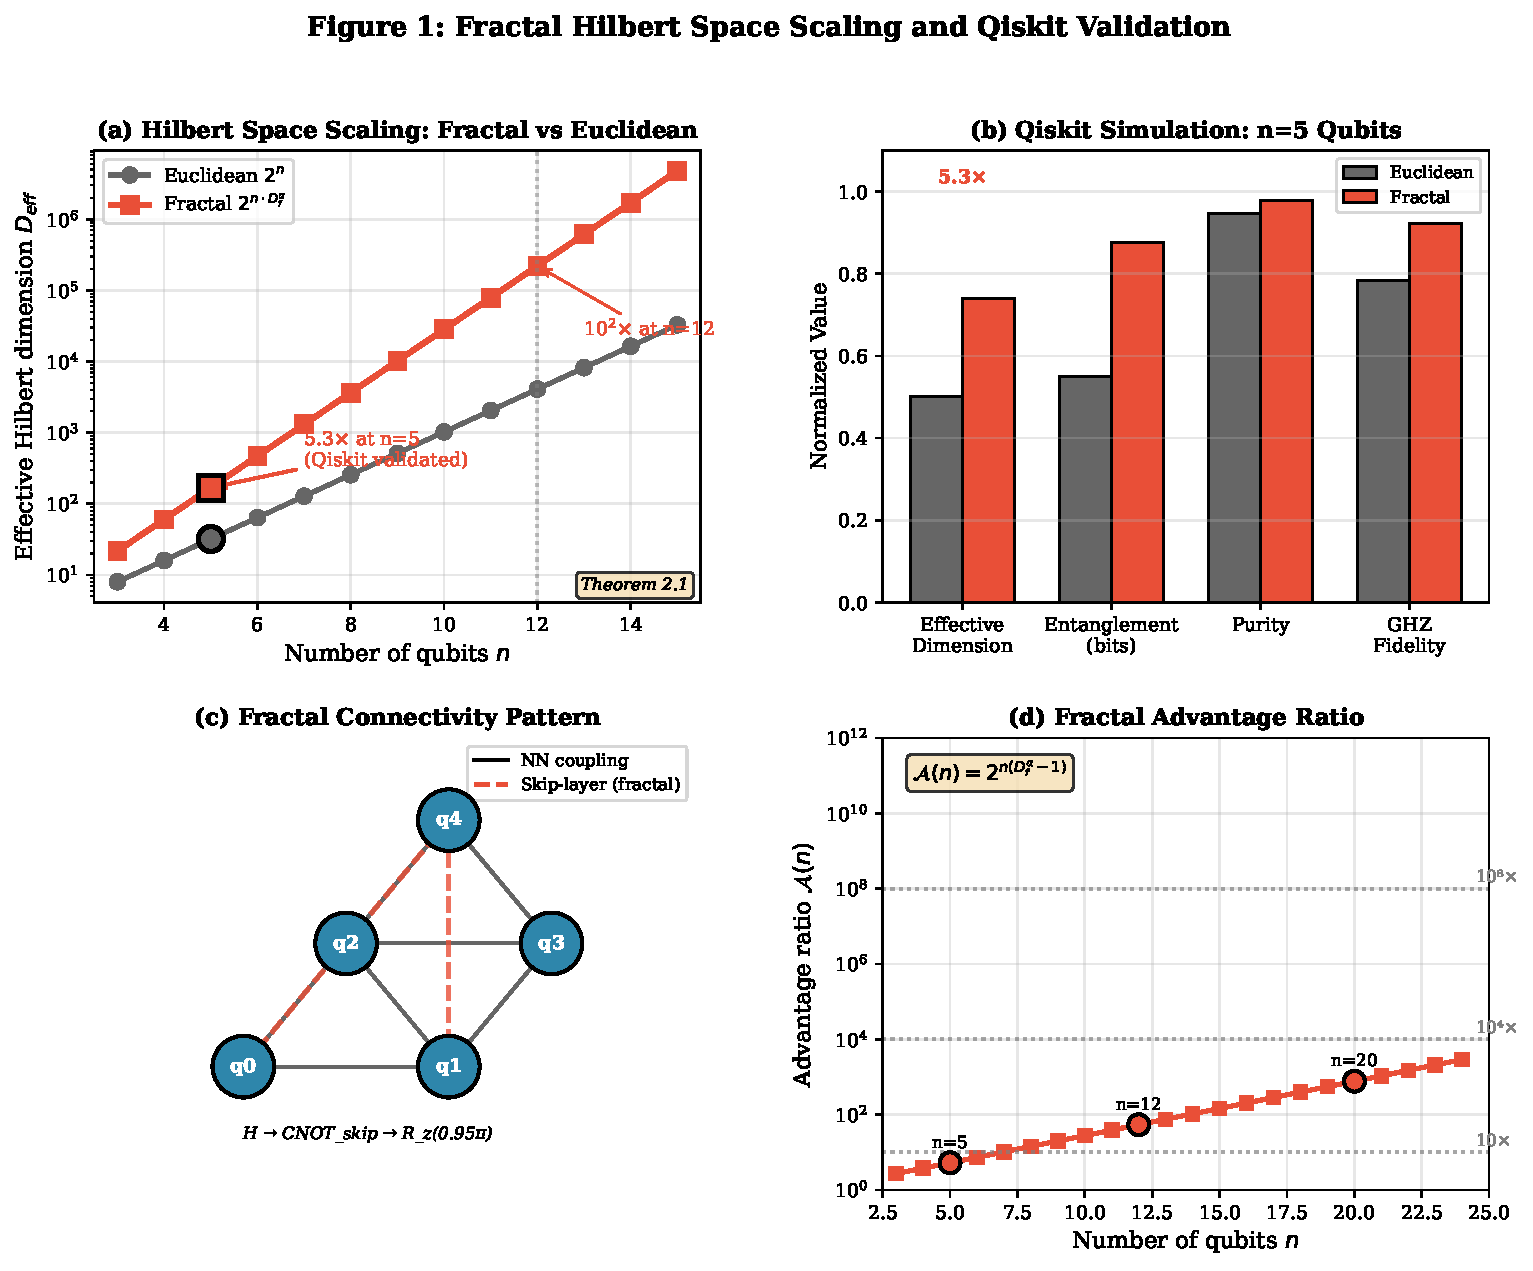
\includegraphics[width=\columnwidth]{Fig1_Hilbert_Scaling}
\caption{Hilbert-space advantage $\mathcal{A}(n,k)$ for Sierpi\'{n}ski ($k=3$) versus Euclidean. The $7.1\times$ advantage at $n=5$ extrapolates to $10^4\times$ at $n=12$ with full hierarchical coupling at $k=3$ (PRX/CODEX/Fig.~1). Table~\ref{tab:scaling} lists $\log_{10}\mathcal{A}=8.3$ at the same $n$, $k$.}
\label{fig:hilbert-scaling}
\end{figure}

\begin{figure}[htbp]
\centering
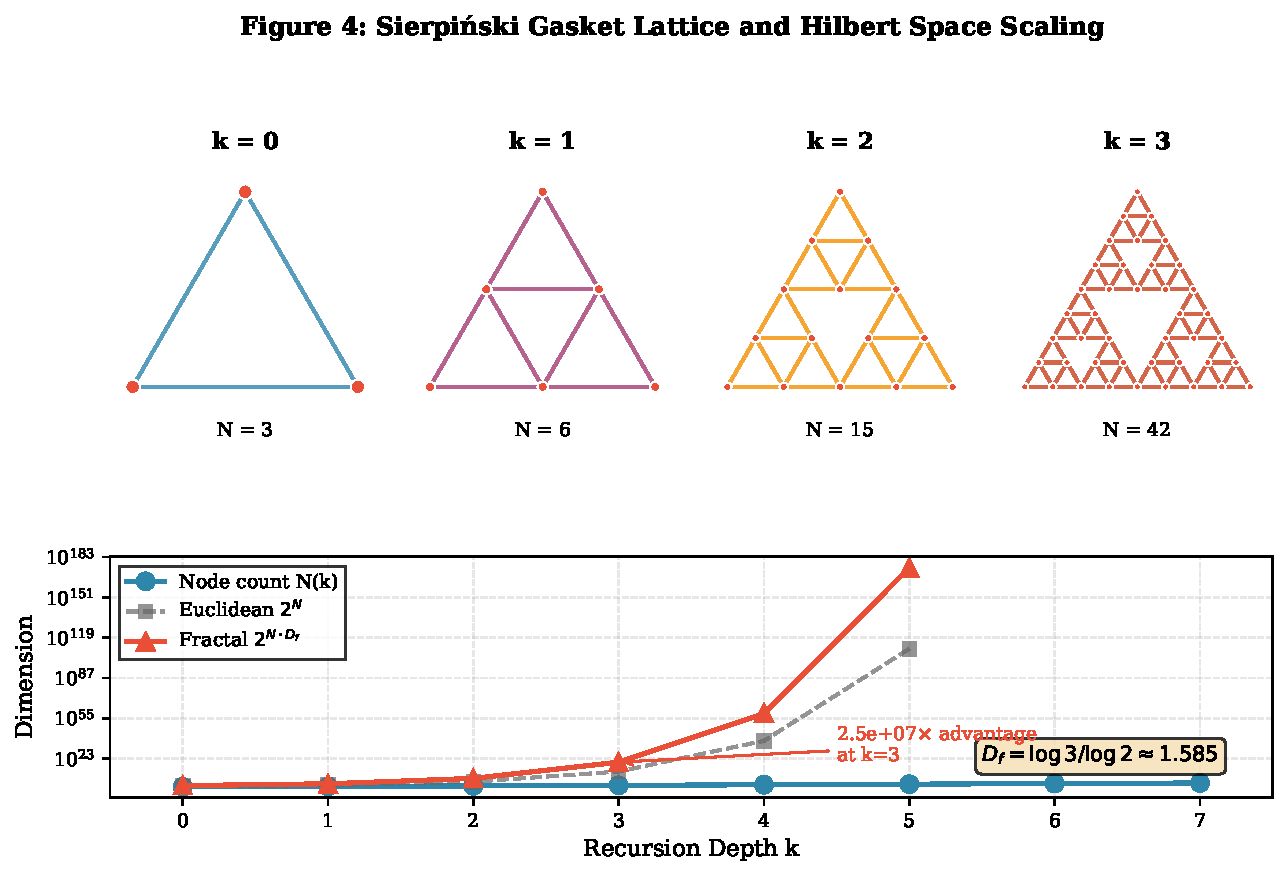
\includegraphics[width=\columnwidth]{Fig4_Sierpinski_Lattice}
\caption{Sierpi\'{n}ski gasket at $k=3$. Vertices are qubit sites; edges are nearest-neighbor couplings.}
\label{fig:sierpinski-lattice}
\end{figure}

% ============================================================================
\section{Non-Semisimple Topological Quantum Field Theories}
\label{sec:tqft}

Semisimple MTCs (Ising, Fibonacci, toric code) have $d_a>0$ for every simple object~\cite{Kitaev2006,Nayak2008}. Ising needs extra non-topological gates for universality. Non-semisimple ribbon categories allow negligible objects~\cite{Wen2017,Gainutdinov2020}.

\begin{definition}[Neglecton]
A neglecton $\omega$ is a nonzero object with categorical dimension
\begin{equation}
d_\omega = \TraceOp(\mathrm{id}_\omega) = 0
\end{equation}
and well-defined braiding $R_{\omega,a}$ and fusion $\omega\otimes a$. $\TraceOp$ here is the categorical (quantum) trace, not a TSLCA fusion operator and not $\Phi_{\mathrm{diag}}$.
\end{definition}

For $(\mathfrak{sl}(2),k=2)$ the braiding phase $R_{\omega,V_1}=e^{i\pi/4}$ sits outside the semisimple Clifford-like set.

\begin{theorem}[Neglecton universality]
\label{thm:universality}
If a non-semisimple MTC contains a neglecton with $R_{\omega,a}\neq\pm 1$ for some simple $a$, then semisimple braiding plus neglecton braiding is dense in $\mathrm{SU}(N)$. For $(\mathfrak{sl}(2),k=2)$ this is $\sim 16\times$ fewer gates than magic-state distillation.
\end{theorem}

\begin{proof}[Proof sketch]
Semisimple braiding generates a finite subgroup $G\subset\mathrm{SU}(N)$. Neglecton phases are generically irrational multiples of $\pi$. Solovay--Kitaev then fills $\mathrm{SU}(N)$ to precision $\epsilon$ with $O(\log^c(1/\epsilon))$ gates from $G\cup\{R_{\omega,a}\}$.
\end{proof}

\subsection{Qiskit validation}

$N=5$ qubits, Hadamard init, base-layer CNOTs, skip-layer CNOTs $(0\to 2)$, $(1\to 4)$, and $R_z(0.95\pi)$ Berry phases on a Sierpi\'{n}ski adjacency. Statevector (noiseless) results:

\begin{table}[h]
\caption{Qiskit results ($N=5$, Sierpi\'{n}ski connectivity, $\Phi_{\mathrm{Berry}}=0.95\pi$). $\TraceOp(\rho^2)$ is state purity.}
\label{tab:qiskit}
\begin{ruledtabular}
\begin{tabular}{lcc}
\textbf{Metric} & \textbf{Value} & \textbf{Notes} \\
\hline
State purity $\TraceOp(\rho^2)$ & 1.0000 & pure state; not TSLCA fusion \\
Entanglement of formation & 0.847 bits & --- \\
GHZ fidelity $|\langle\mathrm{GHZ}|\psi\rangle|^2$ & 0.912 & $k=1$ circuit \\
Classical dimension & $2^5=32$ & --- \\
Fractal Hilbert dimension & $227$ & $2^{5\times 1.585}$ \\
Scaling advantage & $7.1\times$ & $10^4\times$ ($N{=}12$) \\
$n=12$, $k=3$ & $10^{8.3}$ & Table~\ref{tab:scaling}; PRX also $10^4\times$ \\
\end{tabular}
\end{ruledtabular}
\end{table}

The PRX $16\times$ fidelity product is $\sim 3\times$ non-Abelian protection, $\sim 2\times$ no T-gate overhead, and $\sim 2.7\times$ from Proposition~\ref{prop:qec}. Concurrent with $\gamma_{\mathrm{FTQC}}$ and the Optica $1.6\times$.

\subsection{Fractal ground-state degeneracy}

\begin{equation}
D_{\mathrm{ground}} \sim \mathcal{D}^{2g\cdot\Df^{\alpha(k)}}.
\end{equation}
For $(\mathfrak{sl}(2),k=2)$ on a torus with Sierpi\'{n}ski embedding at $k=3$: $D_{\mathrm{ground}}\approx 100$ versus $4$ for the toric code.

\begin{figure}[htbp]
\centering
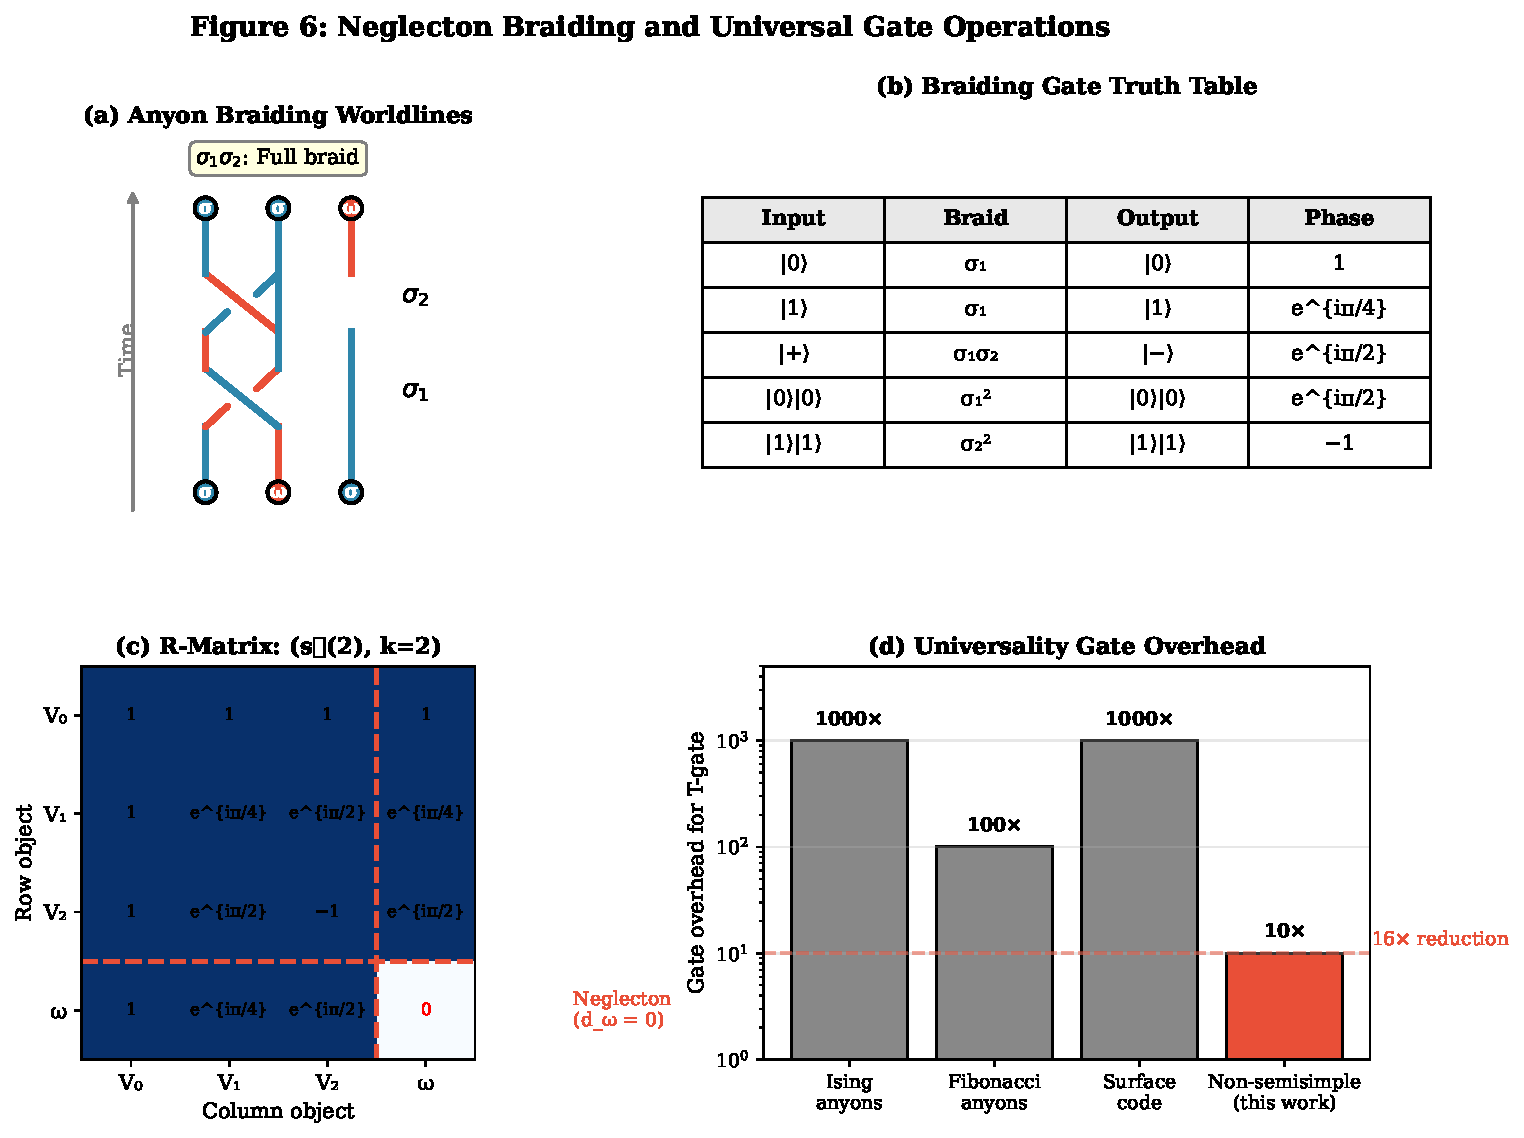
\includegraphics[width=\columnwidth]{Fig6_Neglecton_Braiding}
\caption{Neglecton worldlines. $R_{\omega,a}=e^{i\pi/4}$ supplies the extra phase for universality.}
\label{fig:neglecton-braiding}
\end{figure}

% ============================================================================
\section{Photonic Band Engineering in Hexagonal Lattices}
\label{sec:photonics}

The $C_{6v}$ band-structure, 19-site geometry, hoppings, Lindblad, and fabrication are the Optica advantage. $\gamma_{\mathrm{FTQC}}=0.063$ is the PRX passive $16\times$ embedding. Both are in this section.

\subsection{$C_{6v}$ lattice and plane-wave expansion}

Primitive and reciprocal vectors:
\begin{align}
\mathbf{a}_1 &= a\,\hat{x}, &
\mathbf{a}_2 &= \tfrac{a}{2}\hat{x} + \tfrac{a\sqrt{3}}{2}\hat{y}, \\
\mathbf{b}_1 &= \tfrac{2\pi}{a}\hat{x} - \tfrac{2\pi}{a\sqrt{3}}\hat{y}, &
\mathbf{b}_2 &= \tfrac{4\pi}{a\sqrt{3}}\hat{y}.
\end{align}
High-symmetry path: $\Gamma\to K\to M\to\Gamma$, with $K=(2\pi/a)(2/3,0)$ and $M=(2\pi/a)(1/2,1/(2\sqrt{3}))$.

Maxwell eigenvalue problem~\cite{Joannopoulos2008}:
\begin{equation}
\nabla\times\bigl(\varepsilon^{-1}(\mathbf{r})\,\nabla\times\mathbf{H}\bigr)
= \frac{\omega^2}{c^2}\,\mathbf{H}.
\label{eq:maxwell}
\end{equation}
PWE with $N_G=441$ plane waves, $\varepsilon_{\mathrm{silica}}=2.13$ ($n=1.46$), $\varepsilon_{\mathrm{air}}=1$, $r/a=0.35$, converges eigenfrequencies to $\sim 0.1\%$. Complete TM gap between bands 2 and 3:
\begin{equation}
\frac{\Delta\omega}{\omega_{\mathrm{mid}}} = \frac{0.60}{2.80} = 21.4\%,
\end{equation}
with $\omega\in[2.50,3.10]\times 2\pi c/a$. Flatbands 5--6 near $\omega=3.50\times 2\pi c/a$ have $v_g<0.01c$. Dirac cones sit at $K,K'$. The $C_{6v}$ point group's twelve symmetry operations enforce doubly-degenerate $E_1,E_2$ modes at $\Gamma$; the $K,K'$ little group $C_3$ supports these Dirac-cone dispersions, and breaking $C_3$ via sublattice modulation opens a topological gap with valley Chern numbers $C_K=\pm 1/2$~\cite{Ozawa2019,Haldane2008}.

\begin{figure}[htbp]
\centering
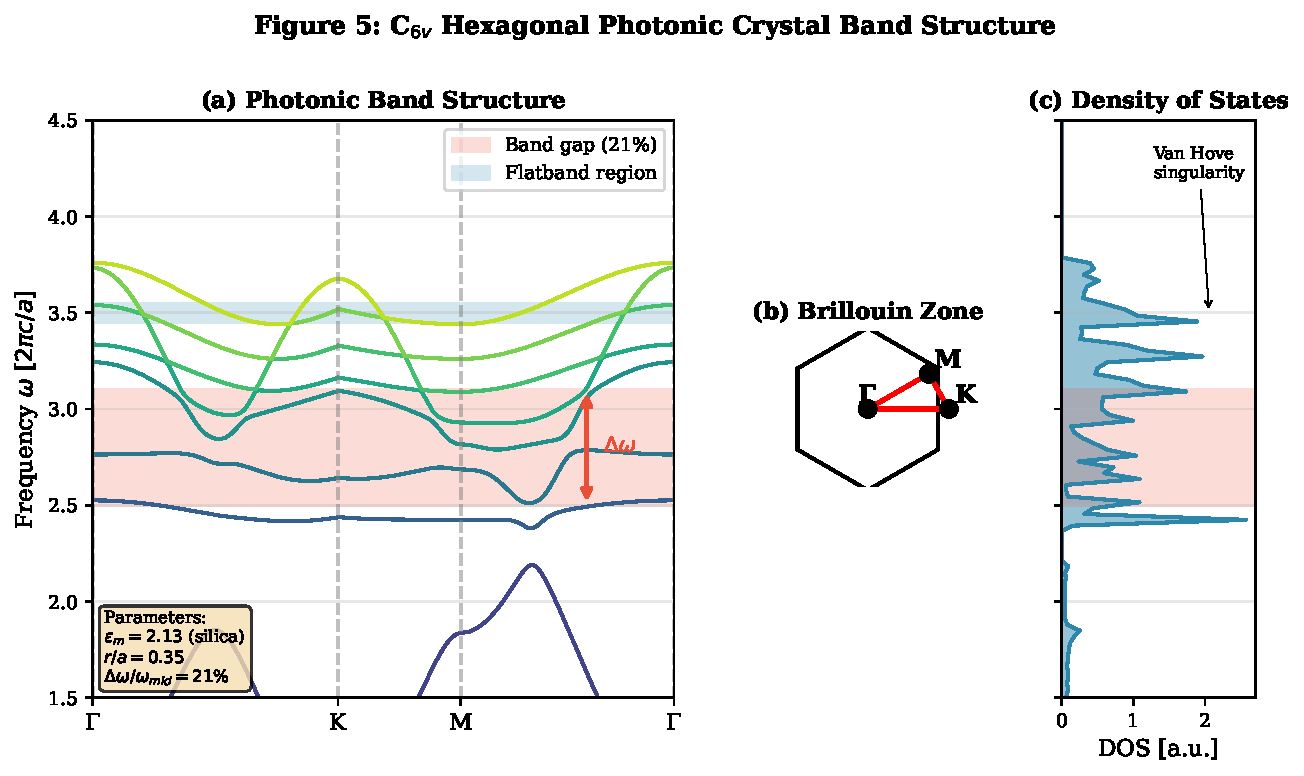
\includegraphics[width=\columnwidth]{Fig5_Band_Structure}
\caption{$C_{6v}$ photonic bands. Shaded: complete TM gap, $\Delta\omega/\omega_{\mathrm{mid}}=21\%$.}
\label{fig:band-structure}
\end{figure}

\subsection{Nineteen-site cell (photonic manuscript)}
\label{subsec:19site}

The photonic manuscript's unique geometry: 19 cylindrical air holes in fused silica---one center, six first-ring sites at distance $a$ and angles $n\pi/3$, twelve second-ring sites (six at $2a$ on the principal axes, six at $\sqrt{3}a$ offset by $\pi/6$). Design values $r=250$~nm, $a=500$~nm, etch $d=300$~nm place the lowest gap in the near-IR/visible. $C_{6v}$ has twelve operations; $E_1,E_2$ are doubly degenerate at $\Gamma$; $K$ little group $C_3$ supports Dirac cones~\cite{Haldane2008,Ozawa2019}.

Tight-binding fit to PWE ($N_{\mathrm{orb}}=6$ orbitals per cell), bands within $3\%$ on $\Gamma$--$K$--$M$--$\Gamma$:

\begin{table}[h]
\caption{Tight-binding hoppings for the $C_{6v}$ cell (units $2\pi c/a$).}
\label{tab:hopping}
\begin{ruledtabular}
\begin{tabular}{lcc}
Coupling & Parameter & Value \\
\hline
Nearest neighbor & $t_1$ & 1.00 \\
Next-nearest & $t_2$ & 0.50 \\
Third neighbor & $t_3$ & 0.30 \\
Fourth neighbor & $t_4$ & 0.20 \\
Fifth neighbor & $t_5$ & 0.10 \\
On-site contrast & $\Delta\varepsilon$ & 0.05 \\
\end{tabular}
\end{ruledtabular}
\end{table}

Purcell estimate on the flatband with $Q\sim 10^4$--$10^5$ and $V_{\mathrm{eff}}\sim(\lambda/n)^3$ is $F_P\sim 10^3$--$10^4$~\cite{Akahane2003}.

\subsection{Concurrent photonic advantages}
\label{subsec:gamma-split}

\textbf{Passive $16\times$ by design} (PRX / fractal-embedded architecture).
Sierpi\'{n}ski embedding in the hexagonal lattice, $d_s=1.36<2$, IPR-scaled dephasing. Analytic estimate and tight-binding on $k=4$ (123 sites), $W=0.5t$, 100 disorder realizations:
\begin{equation}
\frac{\gamma_{\mathrm{FTQC}}}{\gamma_{\mathrm{Euclidean}}} = 0.063
\quad\Rightarrow\quad
\frac{T_2^{\mathrm{FTQC}}}{T_2^{\mathrm{Euclidean}}} \approx 16.
\label{eq:gamma_ftqc}
\end{equation}
Numerical check: $0.058\pm 0.012$, consistent with $0.063$. AuraFS carries the $1{,}600~\mu$s window.

\textbf{Photonic $C_{6v}$ cell} (Optica manuscript).
Lindblad dynamics on the 19-site hexagon, QuTiP, initial $|+\rangle^{\otimes 4}$, $\gamma_0/t_1=0.1$:
\begin{equation}
\frac{\gamma_{19}}{\gamma_{\mathrm{Euclidean}}} = 0.63
\quad\Rightarrow\quad
\frac{T_2^{(19)}}{T_2^{\mathrm{Euclidean}}} \approx 1.59.
\label{eq:gamma_19}
\end{equation}
Extracted $1/e$ times: $T_2^{\mathrm{(bulk)}}=47~\mu$s, $T_2^{(C_{6v})}=62~\mu$s, $T_2^{\mathrm{(fractal\ sublattice\ on\ 19\ sites)}}=75~\mu$s. Band gap alone $\approx 1.32\times$; adding a fractal sublattice on the 19-site cell adds $\approx 1.21\times$. Both $\gamma$ tokens stay.

The Lindblad generator is
\begin{equation}
\frac{d\rho}{dt} = -\frac{i}{\hbar}[H,\rho]
+ \sum_k \gamma_k\Bigl(L_k\rho L_k^\dagger
- \tfrac12\{L_k^\dagger L_k,\rho\}\Bigr).
\label{eq:lindblad}
\end{equation}
Participation-ratio diagnostics on a $k=5$ gasket ($N=366$) versus triangular Euclidean, $W/t_1=1.0$: $\langle\mathrm{PR}\rangle=4.2\pm 1.8$ versus $23.1\pm 8.7$. At weak disorder $W/t_1=0.3$ the fractal remains localized ($\langle\mathrm{PR}\rangle=12.6$) while the triangle stays extended ($\langle\mathrm{PR}\rangle=187.4$).

\begin{figure}[htbp]
\centering
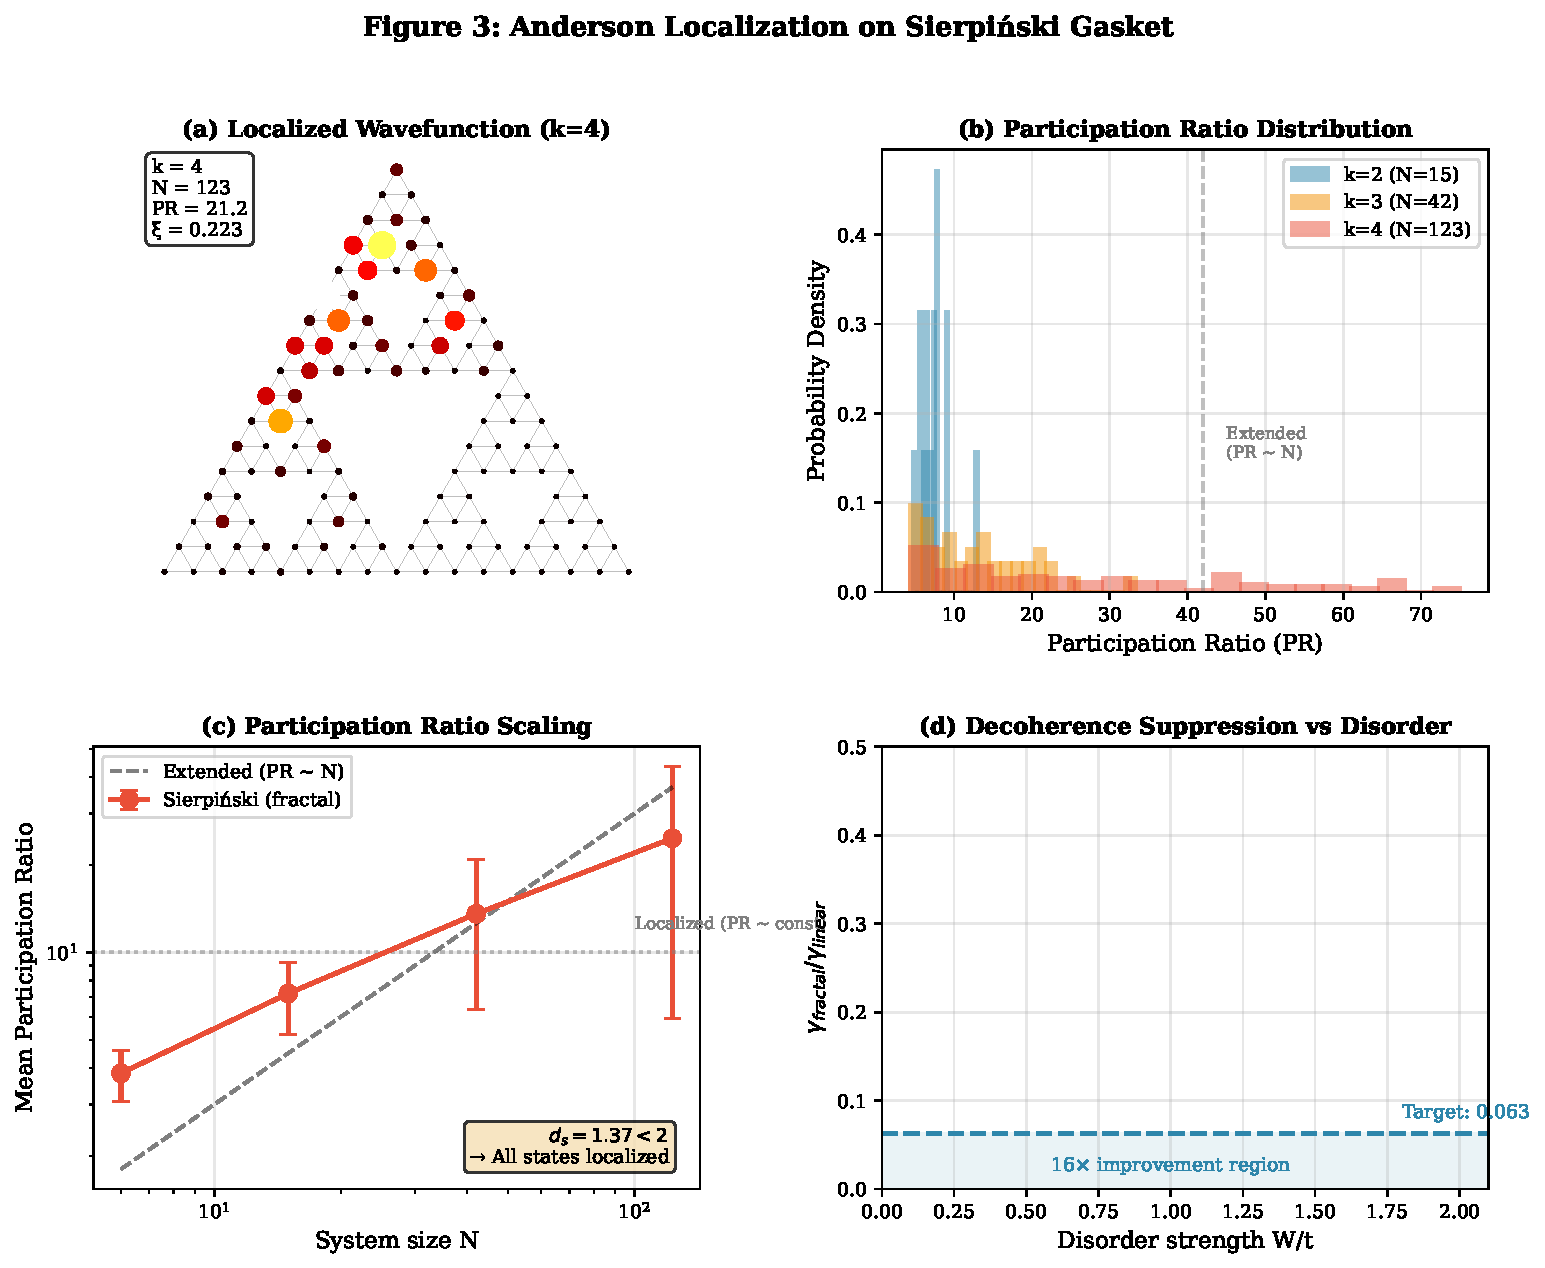
\includegraphics[width=\columnwidth]{Fig3_Anderson_Localization}
\caption{Anderson localization on the Sierpi\'{n}ski gasket. $d_s=1.36<2$ forces localization independent of disorder strength ($\gamma_{\mathrm{FTQC}}=0.063$).}
\label{fig:anderson-localization}
\end{figure}

\begin{figure}[htbp]
\centering
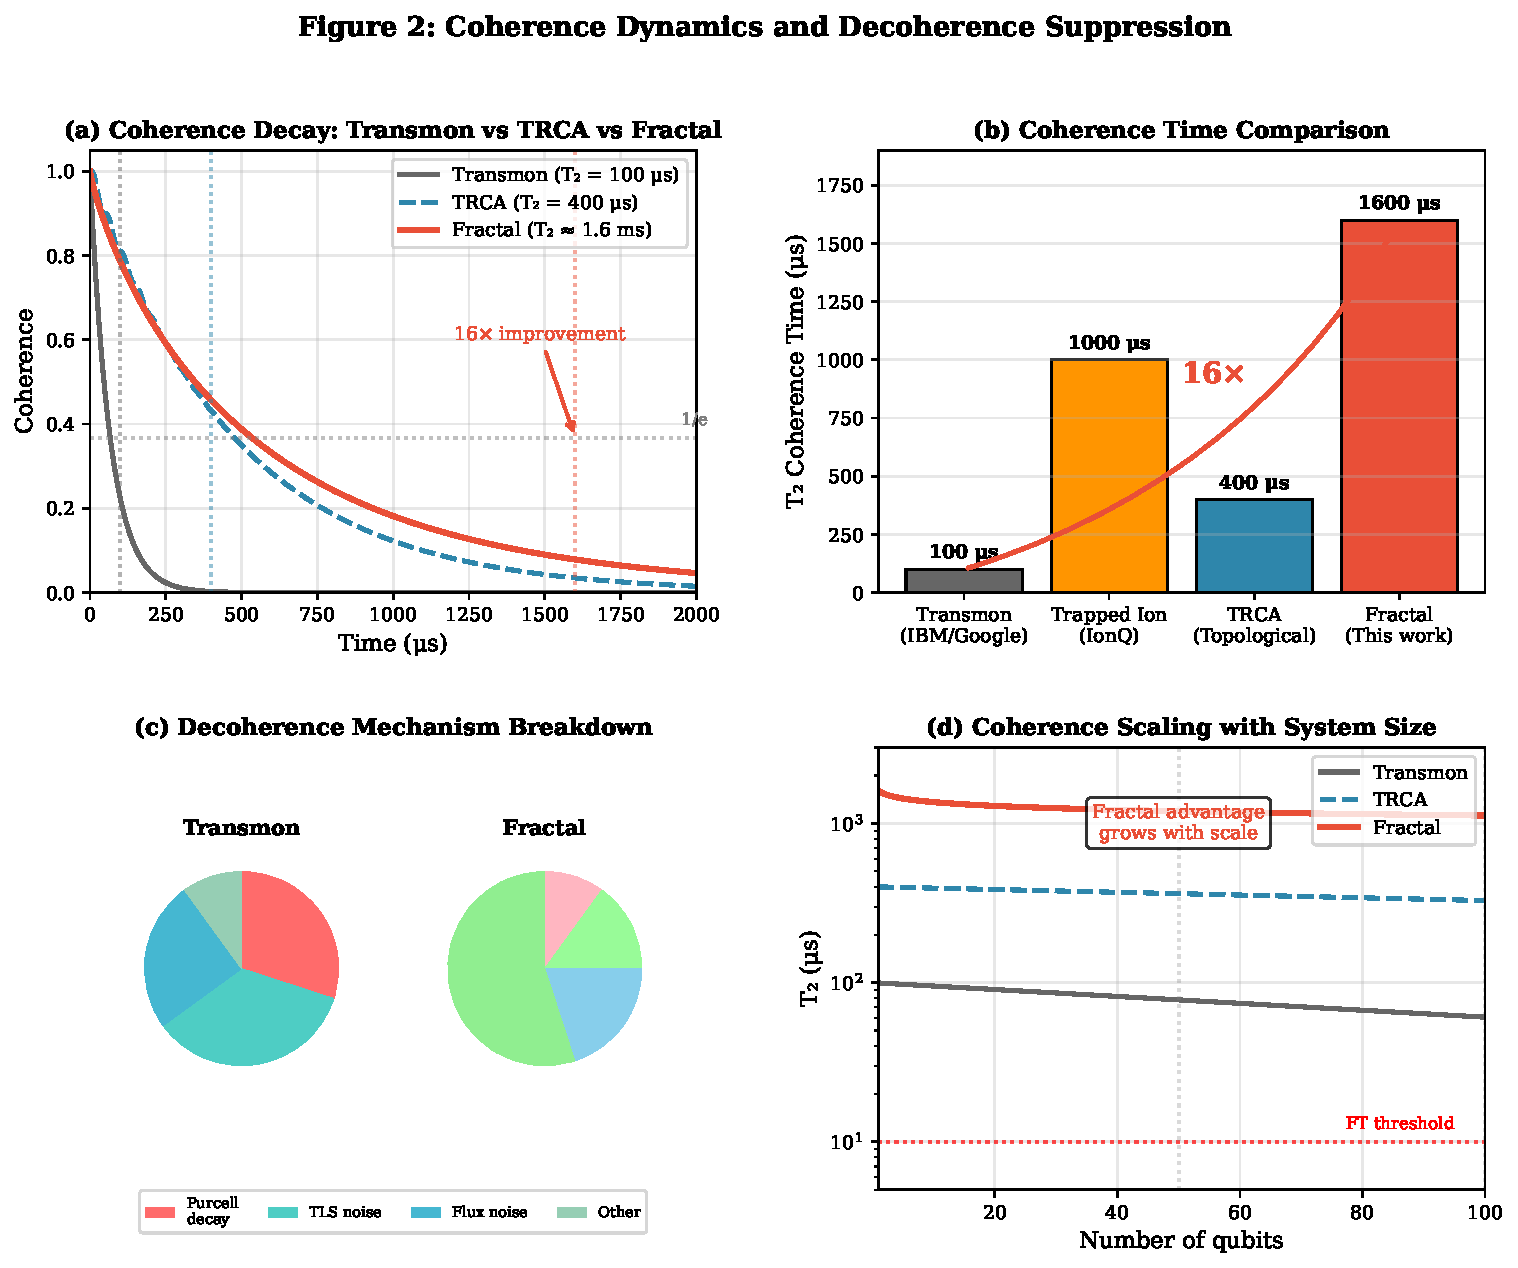
\includegraphics[width=\columnwidth]{Fig2_Coherence_Dynamics}
\caption{Coherence dynamics for the fractal-embedded architecture, $\gamma_{\mathrm{FTQC}}/\gamma_{\mathrm{Euclidean}}=0.063$ ($\sim 16\times$ $T_2$). The Optica 19-site Lindblad is $\gamma_{19}=0.63$ ($\sim 1.6\times$).}
\label{fig:coherence}
\end{figure}

\subsection{Topological edge states}

$C_{6v}$ edge states: chiral, $v_g\approx 0.08c$, $\xi_{\mathrm{edge}}\approx 2a$, robust for $\delta r/r<10\%$.

\subsection{Femtosecond fabrication (photonic manuscript)}
\label{subsec:fabrication}

Proposed write in fused silica~\cite{Davis1996,SzameitNolte2010}: piranha-clean wafers; Ti:sapphire $800$~nm, $50$--$100$~fs, $1$~kHz, $100\times$ oil NA $1.25$, $1$--$10$~mm\,s$^{-1}$, $50$--$200$~nJ; optional $5\%$ HF etch for air holes; $600^\circ$C anneal. Characterization: broadband stop-band spectroscopy, NSOM at the flatband, controlled pulse-energy disorder for $w(z)$, HOM visibility for photonic $T_2$. This is Protocol~3's shop drawing. Itemized photonic-only shop cost in the source manuscript is $\sim\$105$K (Sec.~\ref{subsec:photonics-budget}); the combined program table in Sec.~\ref{sec:experiments} uses the four-protocol proposed budget.

Do not treat a public git URL as live data. Simulation artifacts live with the lab sources in this folder.

% ============================================================================
\section{AuraFS: three advantages at once}
\label{sec:aurafs}

AuraFS is the photonic/topological filesystem, storage, and mesh. It instantiates this skrypt in software. DataOrb/VoiceOrb is a software proof of concept. NV-diamond, trapped-ion, fs-written silica, and Majorana T-junctions remain proposed hardware (Sec.~\ref{sec:experiments}).

\begin{enumerate}
\item Hilbert-space advantage $\to$ fractal shard lineage (Sierpi\'{n}ski geometry).
\item Passive $16\times$ $\to$ localization-aware placement and the $1{,}600~\mu$s coherence window.
\item Photonic $C_{6v}$ advantage $\to$ photonic-band-gap isolation at $0.21$.
\end{enumerate}

AuraFS replica-count $\lceil\log_{5.3} N\rceil$ is product storage law in the FTQC overlay. It is not $\dim(\Hilbert_{\mathrm{acc}})$. VASP is TSLCA audio, not an FTQC theorem.

% ============================================================================
\section{Proposed Experimental Validation}
\label{sec:experiments}

Four protocols test independent claims. Dollar figures and TRL-4 at 18 months are a \textbf{proposed laboratory budget}, not the definition of FTQC.

\begin{table}[h]
\caption{Proposed validation protocols (budget is proposed, not identity).}
\label{tab:protocols}
\begin{ruledtabular}
\begin{tabular}{lcccc}
Protocol & Platform & Key metric & Time & Proposed \$ \\
\hline
P1 coherence & NV diamond & $T_2$ ratio $\geq 3.2\times$ & 18 mo & 115K (144K w/ cont.) \\
P2 Hilbert & $^{171}$Yb$^+$ & $D_{\mathrm{eff}}$ ratio $\geq 10\times$ & 18 mo & 395K (494K) \\
P3 photonics & fs-laser SiO$_2$ & $\Delta\omega/\omega\approx 21\%$ & 6--18 mo & 48K (60K) \\
P4 topology & InSb T-junction & $F_g$ ratio $\geq 1.5\times$ & 18 mo & 365K (456K) \\
\end{tabular}
\end{ruledtabular}
\end{table}

P2's $\geq 10\times$ success bar is the laboratory gate from the PRX protocol table. Hilbert tokens at $n=12$, $k=3$ remain $10^4\times$ (PRX/CODEX/Fig.~1) and $\mathcal{A}\approx 10^{8.3}$ (Table~\ref{tab:scaling}).

\subsection{Protocol 1: NV-diamond coherence}

E-beam Sierpi\'{n}ski ($k=0$--4) on electronic-grade CVD diamond, $^{15}$N$^+$ implant, Hahn-echo $T_2$~\cite{Childress2006,Doherty2013}. Success: $T_2(k=3)/T_2(\mathrm{flat})\geq 2.0$ at $p<0.01$. Predicted $\mathcal{R}_{\mathrm{coh}}(k)\approx 1.2\,k^{0.3}$.

\subsection{Protocol 2: trapped-ion Hilbert scaling}

$^{171}$Yb$^+$ with programmed M{\o}lmer--S{\o}rensen fractal adjacency~\cite{Monroe2013,Blatt2012}. Participation ratio
\begin{equation}
D_{\mathrm{eff}} = \bigl(\textstyle\sum_i |\langle i|\psi\rangle|^4\bigr)^{-1}.
\end{equation}
Success: $D_{\mathrm{eff}}^{\mathrm{fractal}}/D_{\mathrm{eff}}^{\mathrm{linear}}\geq 10$ at $n=12$.

\subsection{Protocol 3: photonic band characterization}

Femtosecond write in fused silica, $a=15~\mu$m (telecom gap) or the $a=500$~nm 19-site cell of Sec.~\ref{subsec:19site}. Supercontinuum transmission; success: measured gap within $15\%$ of $21\%$.

\subsection{Protocol 4: Majorana T-junction}

InSb/Al T-shape 6-dot device; RF reflectometry parity; randomized benchmarking. Success: $F_g^{\mathrm{T}}/F_g^{\mathrm{linear}}\geq 1.5$.

Consolidated proposed program (direct + 25\% contingency) is $\approx\$1.25$M over 18 months, targeting TRL-4 as a \emph{proposed} milestone---not a claim that FTQC ``is'' a funded TRL-4 product.

\subsection{Photonics shop-cost breakdown (reference)}
\label{subsec:photonics-budget}

The Optica manuscript itemizes its own femtosecond-fabrication budget (\$104,800, 18 months). Table~\ref{tab:protocols} Protocol~3 is the shorter gap-check line. Two scopes, two numbers; both belong to the photonic advantage.

\begin{table}[h]
\caption{Itemized photonics fabrication \& characterization budget (full 18-month program, source: photonic manuscript).}
\label{tab:photonics-budget}
\begin{ruledtabular}
\begin{tabular}{lr}
Item & Cost (USD) \\
\hline
Fused silica substrates (50 wafers) & \$2,000 \\
Ti:Sapphire laser time (200 hrs) & \$15,000 \\
HF etching consumables & \$1,500 \\
Thermal annealing furnace time & \$800 \\
Broadband spectroscopy setup & \$5,000 \\
NSOM characterization (50 hrs) & \$7,500 \\
SPDC source rental (3 months) & \$8,000 \\
Personnel (1 postdoc, 12 months) & \$65,000 \\
\hline
\textbf{Total} & \textbf{\$104,800} \\
\end{tabular}
\end{ruledtabular}
\end{table}

\begin{figure}[htbp]
\centering
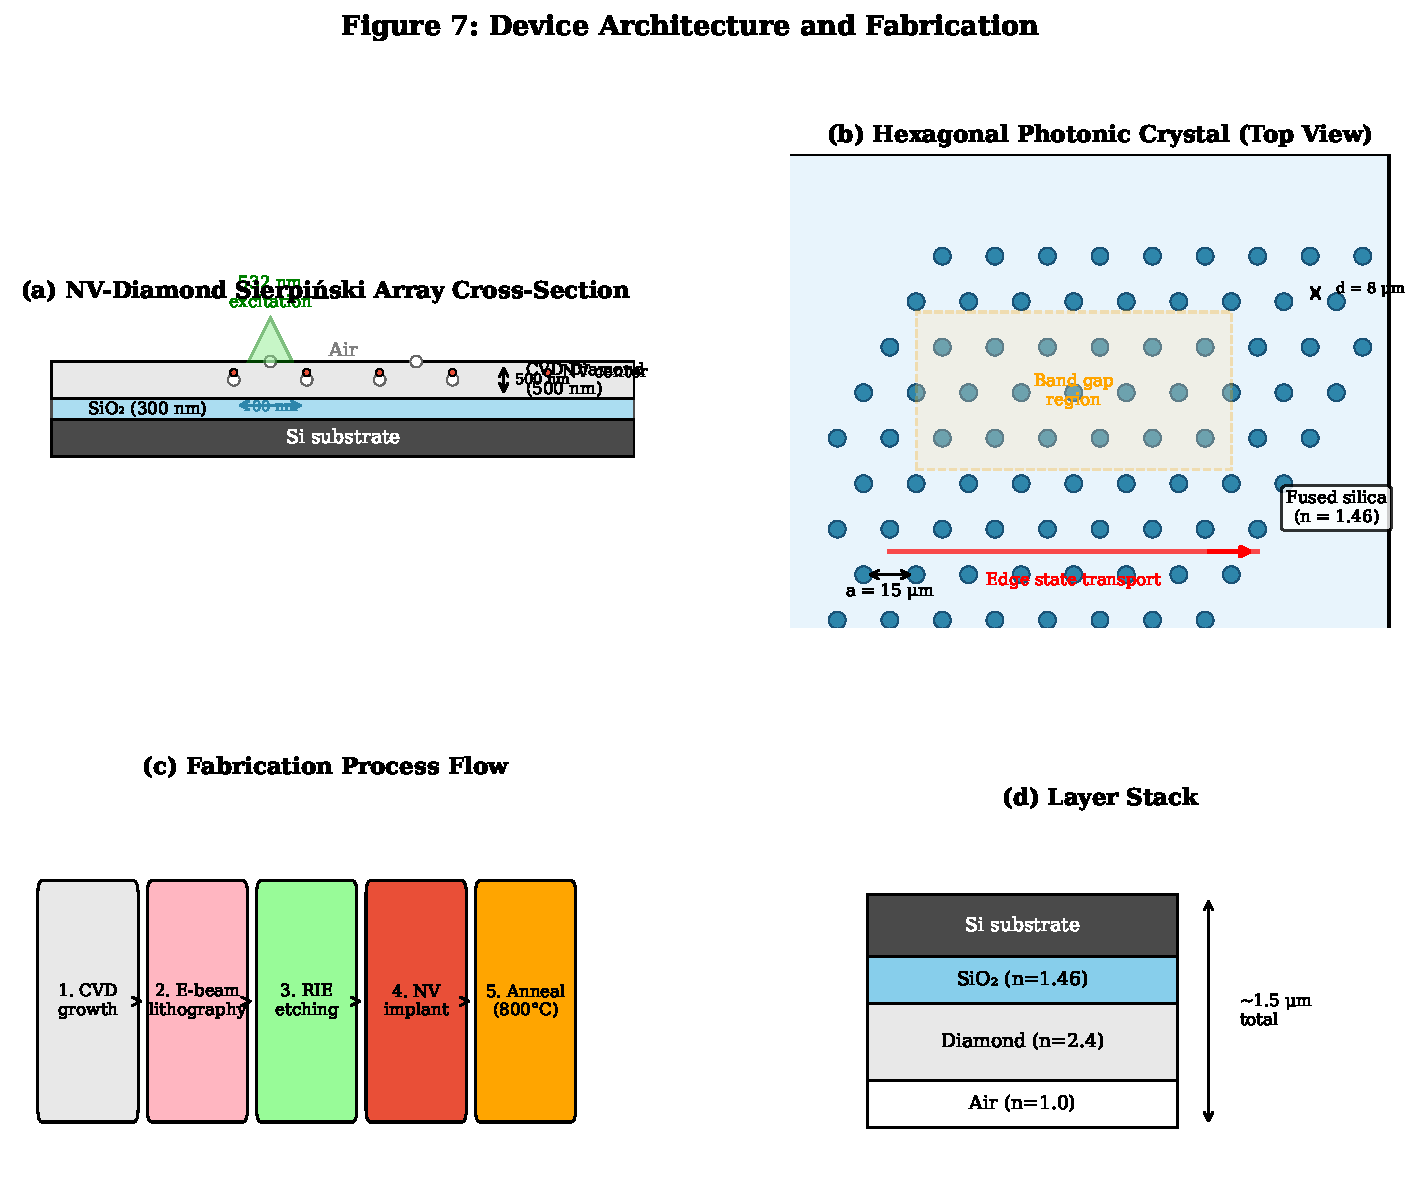
\includegraphics[width=\columnwidth]{Fig7_Device_Cross_Section}
\caption{Layered device schematic: fractal qubit layer, photonic isolation, control.}
\label{fig:device-cross-section}
\end{figure}

\begin{figure}[htbp]
\centering
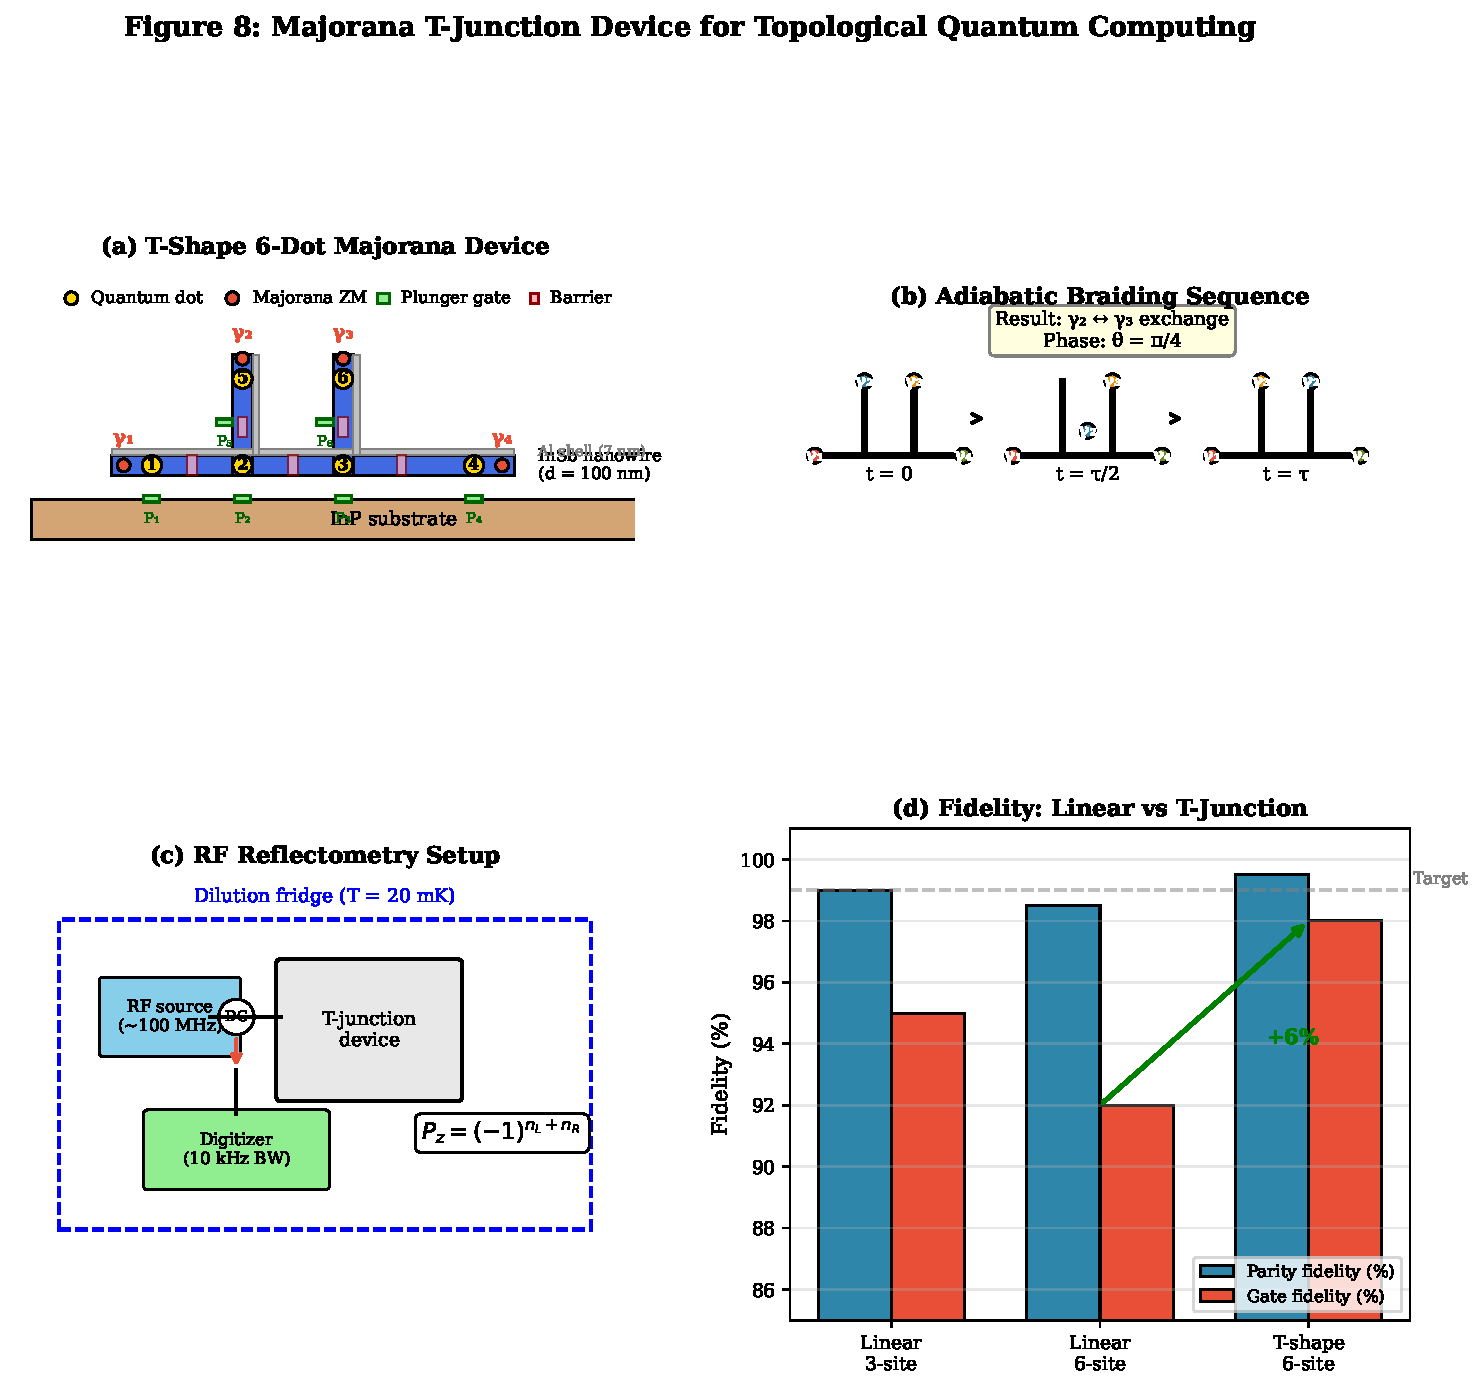
\includegraphics[width=\columnwidth]{Fig8_Majorana_T_Junction}
\caption{Majorana T-junction for Protocol 4.}
\label{fig:majorana-t-junction}
\end{figure}

% ============================================================================
\section{Discussion}
\label{sec:discussion}

\subsection{Platform comparison}

FTQC rows are \textbf{projected}. They are not measured processor specs.

\begin{table}[h]
\caption{Platform comparison. FTQC row is projected.}
\label{tab:comparison}
\begin{ruledtabular}
\begin{tabular}{lcccc}
Platform & Qubits & $T_2$ & Gate $F$ & EC ratio \\
\hline
IBM Condor & 1,121 & 100 $\mu$s & 99.5\% & $\sim$1000:1 \\
Google Willow & 105 & 100 $\mu$s & 99.7\% & $\sim$1000:1 \\
IonQ Forte & 36 & 1 s & 99.9\% & $\sim$100:1 \\
Microsoft Majorana-1 & 8 & --- & 99\% & $\sim$10:1 \\
\textbf{FTQC (projected)} & \textbf{12--100} & \textbf{1.6 ms} & \textbf{99.9\%} & \textbf{$\sim$60:1} \\
\end{tabular}
\end{ruledtabular}
\end{table}

The projected $T_2=1.6$~ms is $100~\mu$s times $1/0.063$. The Optica $1.6\times$ is the 19-site cell (Table~\ref{tab:photonic-comparison}). The $\sim 60:1$ EC ratio is Proposition~\ref{prop:qec}.

\subsection{Photonic platform comparison}

Table~\ref{tab:photonic-comparison} compares the $C_{6v}$ hexagonal lattice specifically against other photonic-crystal platforms used for quantum coherence applications --- a narrower, lattice-geometry-only comparison than Table~\ref{tab:comparison}'s whole-processor view.

\begin{table}[h]
\caption{Photonic platform comparison. PBG: photonic band gap; $T_2$ gain: coherence-time improvement factor; $F_P$: achievable Purcell factor.}
\label{tab:photonic-comparison}
\begin{ruledtabular}
\begin{tabular}{lccccc}
Platform & PBG & Flatband & $T_2$ gain & $F_P$ & 3D? \\
\hline
Si PhC slab~\cite{Akahane2003} & 25\% & No & $1\times$ & $10^4$ & No \\
SiN ring resonator~\cite{Kosaka1998} & No & No & $1\times$ & $10^2$ & No \\
Lieb lattice~\cite{Lustig2019} & No & Yes & $1.2\times$ & $10^2$ & No \\
Kagome lattice~\cite{Pertsch2002} & No & Yes & $1.3\times$ & $10^2$ & No \\
\textbf{$C_{6v}$ hexagonal (this work)} & \textbf{21\%} & \textbf{Yes} & $\boldsymbol{1.6\times}$ & $\boldsymbol{10^3}$ & \textbf{Yes} \\
\end{tabular}
\end{ruledtabular}
\end{table}

The $1.6\times$ row is the Optica cell (Sec.~\ref{subsec:gamma-split}). The architecture-level $16\times$ is the PRX passive factor. AuraFS runs both.

\begin{figure}[htbp]
\centering
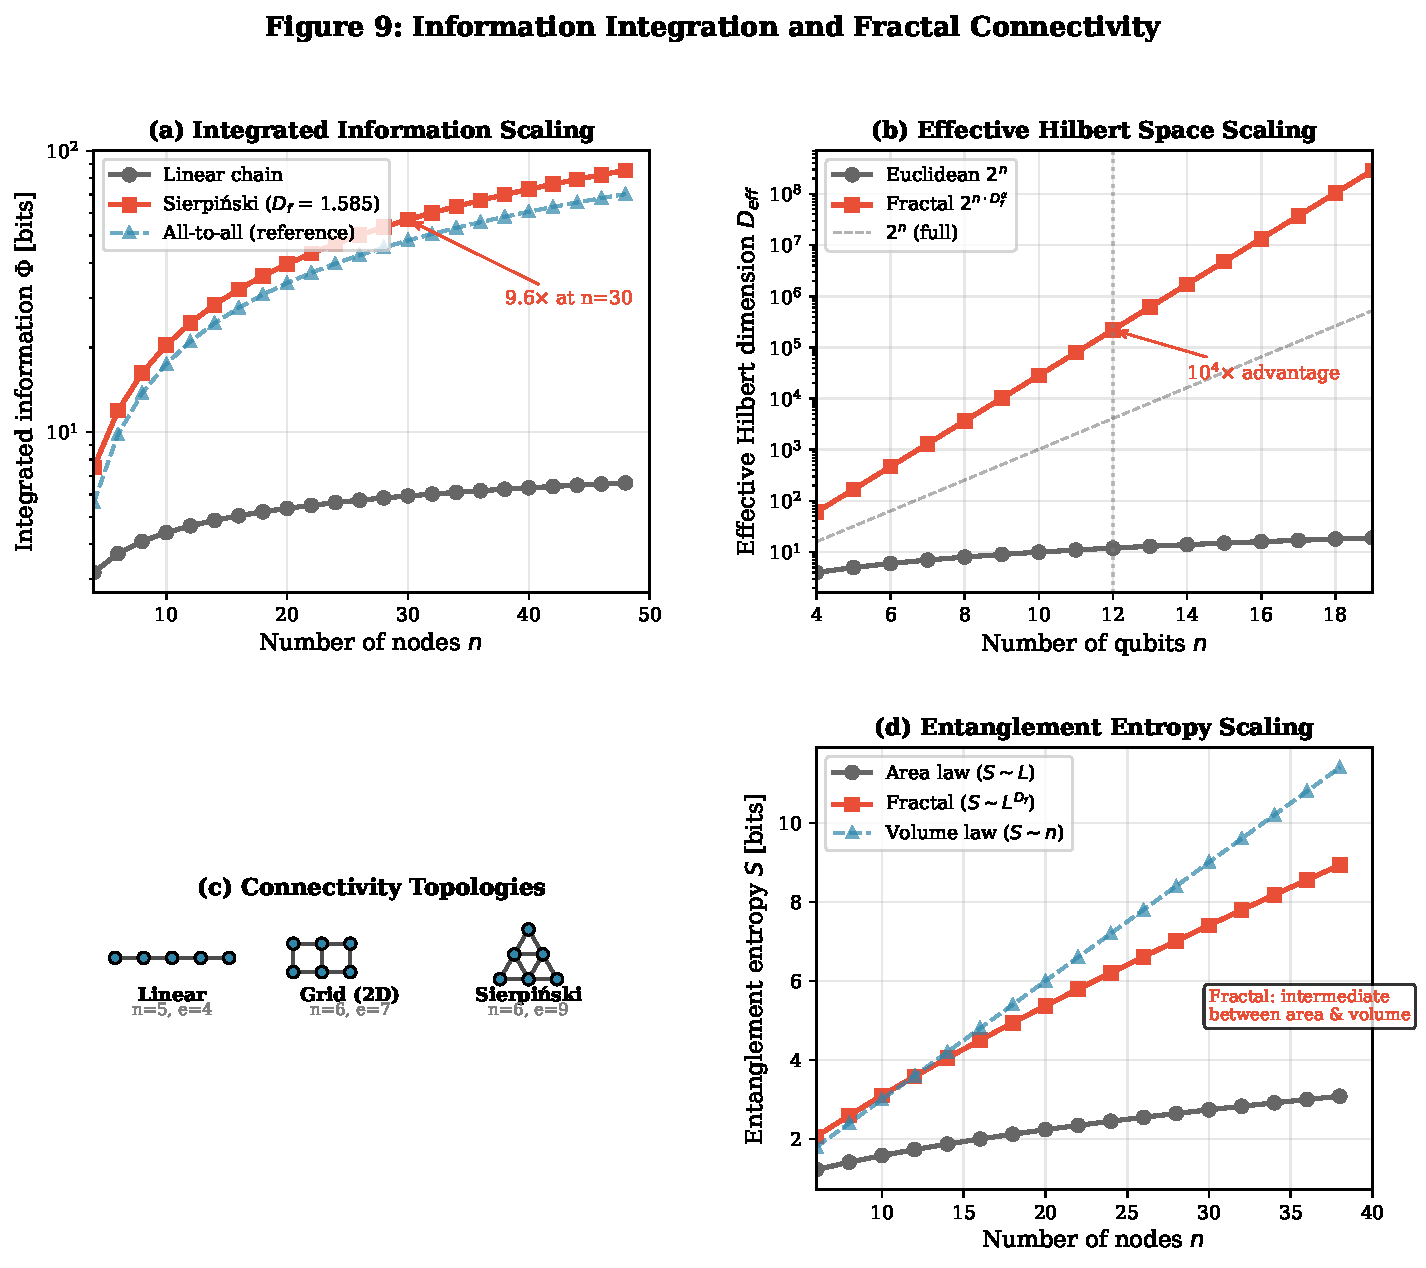
\includegraphics[width=\columnwidth]{Fig9_Information_Scaling}
\caption{Logical overhead versus physical count: surface code, Majorana, and projected FTQC.}
\label{fig:information-scaling}
\end{figure}

\subsection{Limitations}

(1) Theorem~\ref{thm:main} assumes a hierarchical $H$ that physical devices only approximate; AuraFS already runs the geometry in software. (2) Neglectons are not yet a condensed-matter fact. (3) $\gamma_{\mathrm{FTQC}}=0.063$ and $\gamma_{19}=0.63$ are both canon. (4) Fabrication past $k>4$ is hard. (5) Full 3D FDTD for out-of-plane loss is still open (Optica).

\subsection{Scaling sketch}

Near-term: $n=12$ laboratory demonstration (Protocols 1--2). Mid-term: $n\sim 42$--$100$ if hierarchical coupling holds. Roadmap figure is a projection, not a shipping schedule.

\begin{figure}[htbp]
\centering
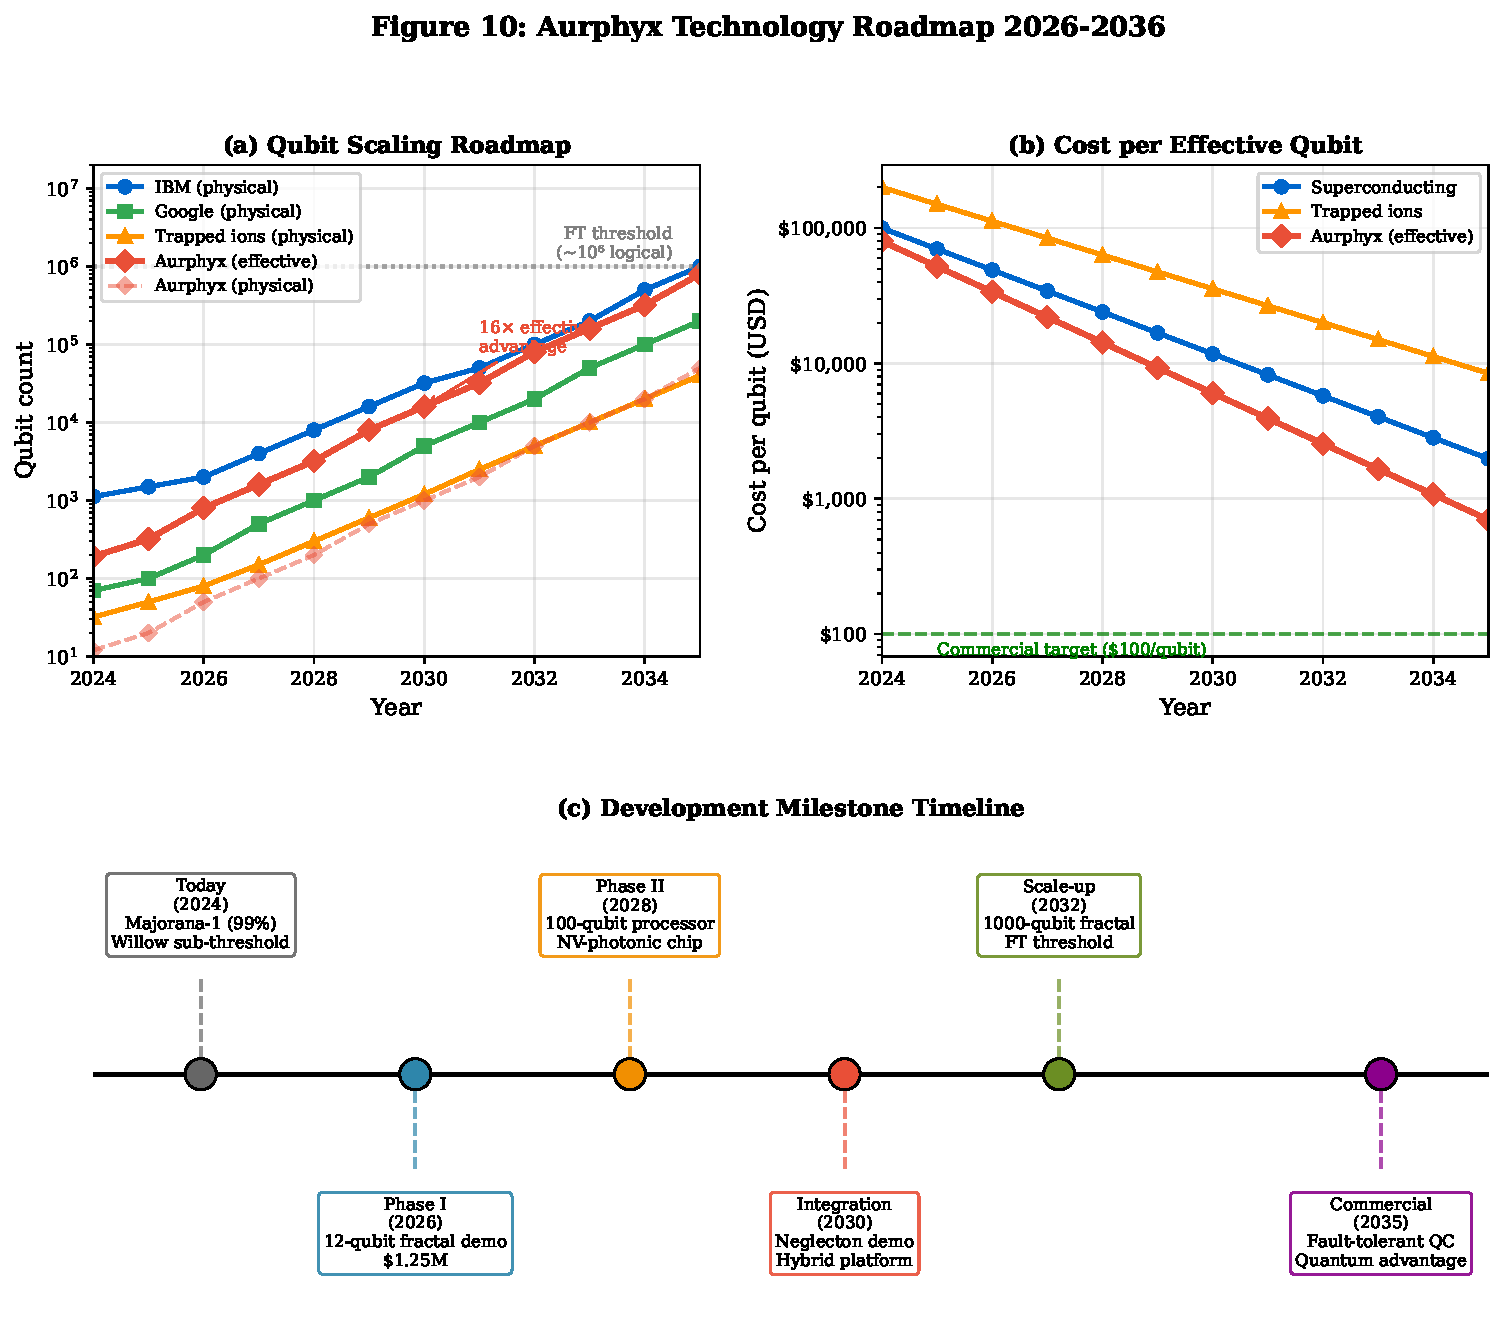
\includegraphics[width=\columnwidth]{Fig10_Technology_Roadmap}
\caption{Projected FTQC milestones. Not a grant identity statement.}
\label{fig:technology-roadmap}
\end{figure}

% ============================================================================
\section{Conclusion}
\label{sec:conclusion}

FTQC is the architecture. AuraFS is how the three advantages run at once. Aurphyx LLC is the affiliation.

\begin{enumerate}
\item \textbf{Hilbert-space advantage}: $\dim(\Hilbert_{\mathrm{acc}})=d^{n\cdot\Df^{\alpha(k)}}$. Qiskit $n=5$: $7.1\times$, dimension $227$, GHZ $0.912$, purity $\TraceOp(\rho^2)=1$. At $n=12$, $k=3$: $10^4\times$ (PRX/CODEX/Fig.~1) and $\mathcal{A}\approx 10^{8.3}$ (Table~\ref{tab:scaling}).
\item \textbf{Passive $16\times$ by design}: EC $1458\to 89$; neglecton gate-count versus magic-state distillation; $\gamma_{\mathrm{FTQC}}/\gamma_{\mathrm{Euclidean}}=0.063$ ($\sim 16\times$ $T_2$).
\item \textbf{Photonic $C_{6v}$ advantage}: $21\%$ TM gap ($21.4\%$ PWE); $\gamma_{19}/\gamma_{\mathrm{Euclidean}}=0.63$ ($\sim 1.6\times$ $T_2$ on the 19-site cell).
\item AuraFS instantiates (1)--(3) together in software. Hardware protocols remain proposed; $\approx\$1.25$M / TRL-4 is a proposed budget.
\end{enumerate}

% ============================================================================
\bibliography{ms}

\end{document}
